\documentclass[a5paper, 10pt]{memoir}

\usepackage{color}
\usepackage[english]{babel}
\usepackage[utf8]{inputenc}
\usepackage{amsmath}
\usepackage{graphicx}
\usepackage[lining]{ebgaramond}
\usepackage{makeidx}
\usepackage{fancyvrb}
\usepackage[backend=biber,style=authoryear,citestyle=numeric-comp,sorting=none,firstinits=true]{biblatex}\addbibresource{main.bib}

\usepackage[textsize=small, linecolor=magenta, bordercolor=magenta,
            backgroundcolor=magenta, colorinlistoftodos]{todonotes}
\usepackage{letltxmacro}
\LetLtxMacro{\oldtodo}{\todo}
\renewcommand{\todo}[1]{{\color{white}\oldtodo{\textsf{#1}}}}

\semiisopage[9]
\checkandfixthelayout

\setlength{\parindent}{0cm}

\usepackage{hyperref}

%\setlength{\parindent}{0cm} % egonw, do we need to have a word about this?
\RecustomVerbatimEnvironment{Verbatim}{Verbatim}{xleftmargin=5mm}

% from: http://www.joachim-breitner.de/blog/archives/519-Nicer-URL-formatting-in-LaTeX.html
% changes look of URLs
\urlstyle{sf}
\makeatletter
    \let\UrlSpecialsOld\UrlSpecials
    \def\UrlSpecials{\UrlSpecialsOld\do\/{\Url@slash}\do\_{\Url@underscore}}%
    \def\Url@slash{\@ifnextchar/{\kern-.11em\mathchar47\kern-.2em}%
        {\kern-.0em\mathchar47\kern-.08em\penalty\UrlBigBreakPenalty}}
        \def\Url@underscore{\nfss@text{\leavevmode \kern.06em\vbox{\hrule\@width.3em}}}
\makeatother

\setsecheadstyle{\Large}
\setsubsecheadstyle{\scshape}
\setsubsubsecheadstyle{\itshape}
\setparaheadstyle{\itshape}

\makeindex

\hyphenation{Java-Script}

\title{A lot of \\ Bioclipse Scripting Language \\ examples \\ (DRAFT)}

\author{E.L. Willighagen, J. Alvarsson}

\begin{document}
\maketitle

\newpage
\pagestyle{plain}
\mbox{}\vfill
{\noindent \textsf{This work is made available under the Creative Commons
Attribution-ShareAlike 4.0 International license.}}
\vskip 5 ex
\begin{center}
	
\includegraphics[width=0.3\textwidth]{ccbysa.png}
\end{center}
\vfill
\newpage

\tableofcontents

\chapter{Introduction}
\begin{refsection}

Just to set the record straight, this book is available under a Creative
Commons~4.0 Attribution ShareAlike license. Therefore, feel free to copy this
book, share it with friends, or extend it with additional code examples.

We will explain some basics of the Bioclipse Scripting Language (\textsc{bsl})
idea~\cite{spjuth2009bioclipse}, and then the following chapters will
describe\index{bsl} functionality available in this language. Each chapter is
written around a particular area. But before we get to scripting let's look at
how to get Bioclipse running!

\section{Downloading, installing and updating Bioclipse}
This section gives a short introduction for how tog get started with Bioclipse
and is mainly cut from the ``Getting started with Bioclipse 2.6'' folder. For
the complete Getting started text see~\ref{BioclipseGettingStarted}.

\subsection{Downloading}
Bioclipse for Windows comes in a couple of different packages. Either as a
\texttt{.zip} file or as an installation program and either as 32 or 64 bit. To
find out if you have 32 or 64 bit in Windows~XP  and Windows~7 right click the
icon named \texttt{My} \texttt{computer} and choose \texttt{properties}. On
Windows~8 you need to go to \texttt{System} \texttt{and} \texttt{Security} and
then \texttt{view} \texttt{basic} \texttt{information} \texttt{about}
\texttt{your} \texttt{computer}.  Normally, the installation program should be
the obvious choice but if, for whatever reason, that doesn't work you can use
the zip file. The Linux version is packaged as a tar.gz file and the Mac
version comes as a .dmg file. These packages are available from:

\vskip 0.5\baselineskip
{\footnotesize \noindent \url{https://sourceforge.net/projects/bioclipse/files/bioclipse2/bioclipse2.6.1/}.}

\begin{center}
    \fbox{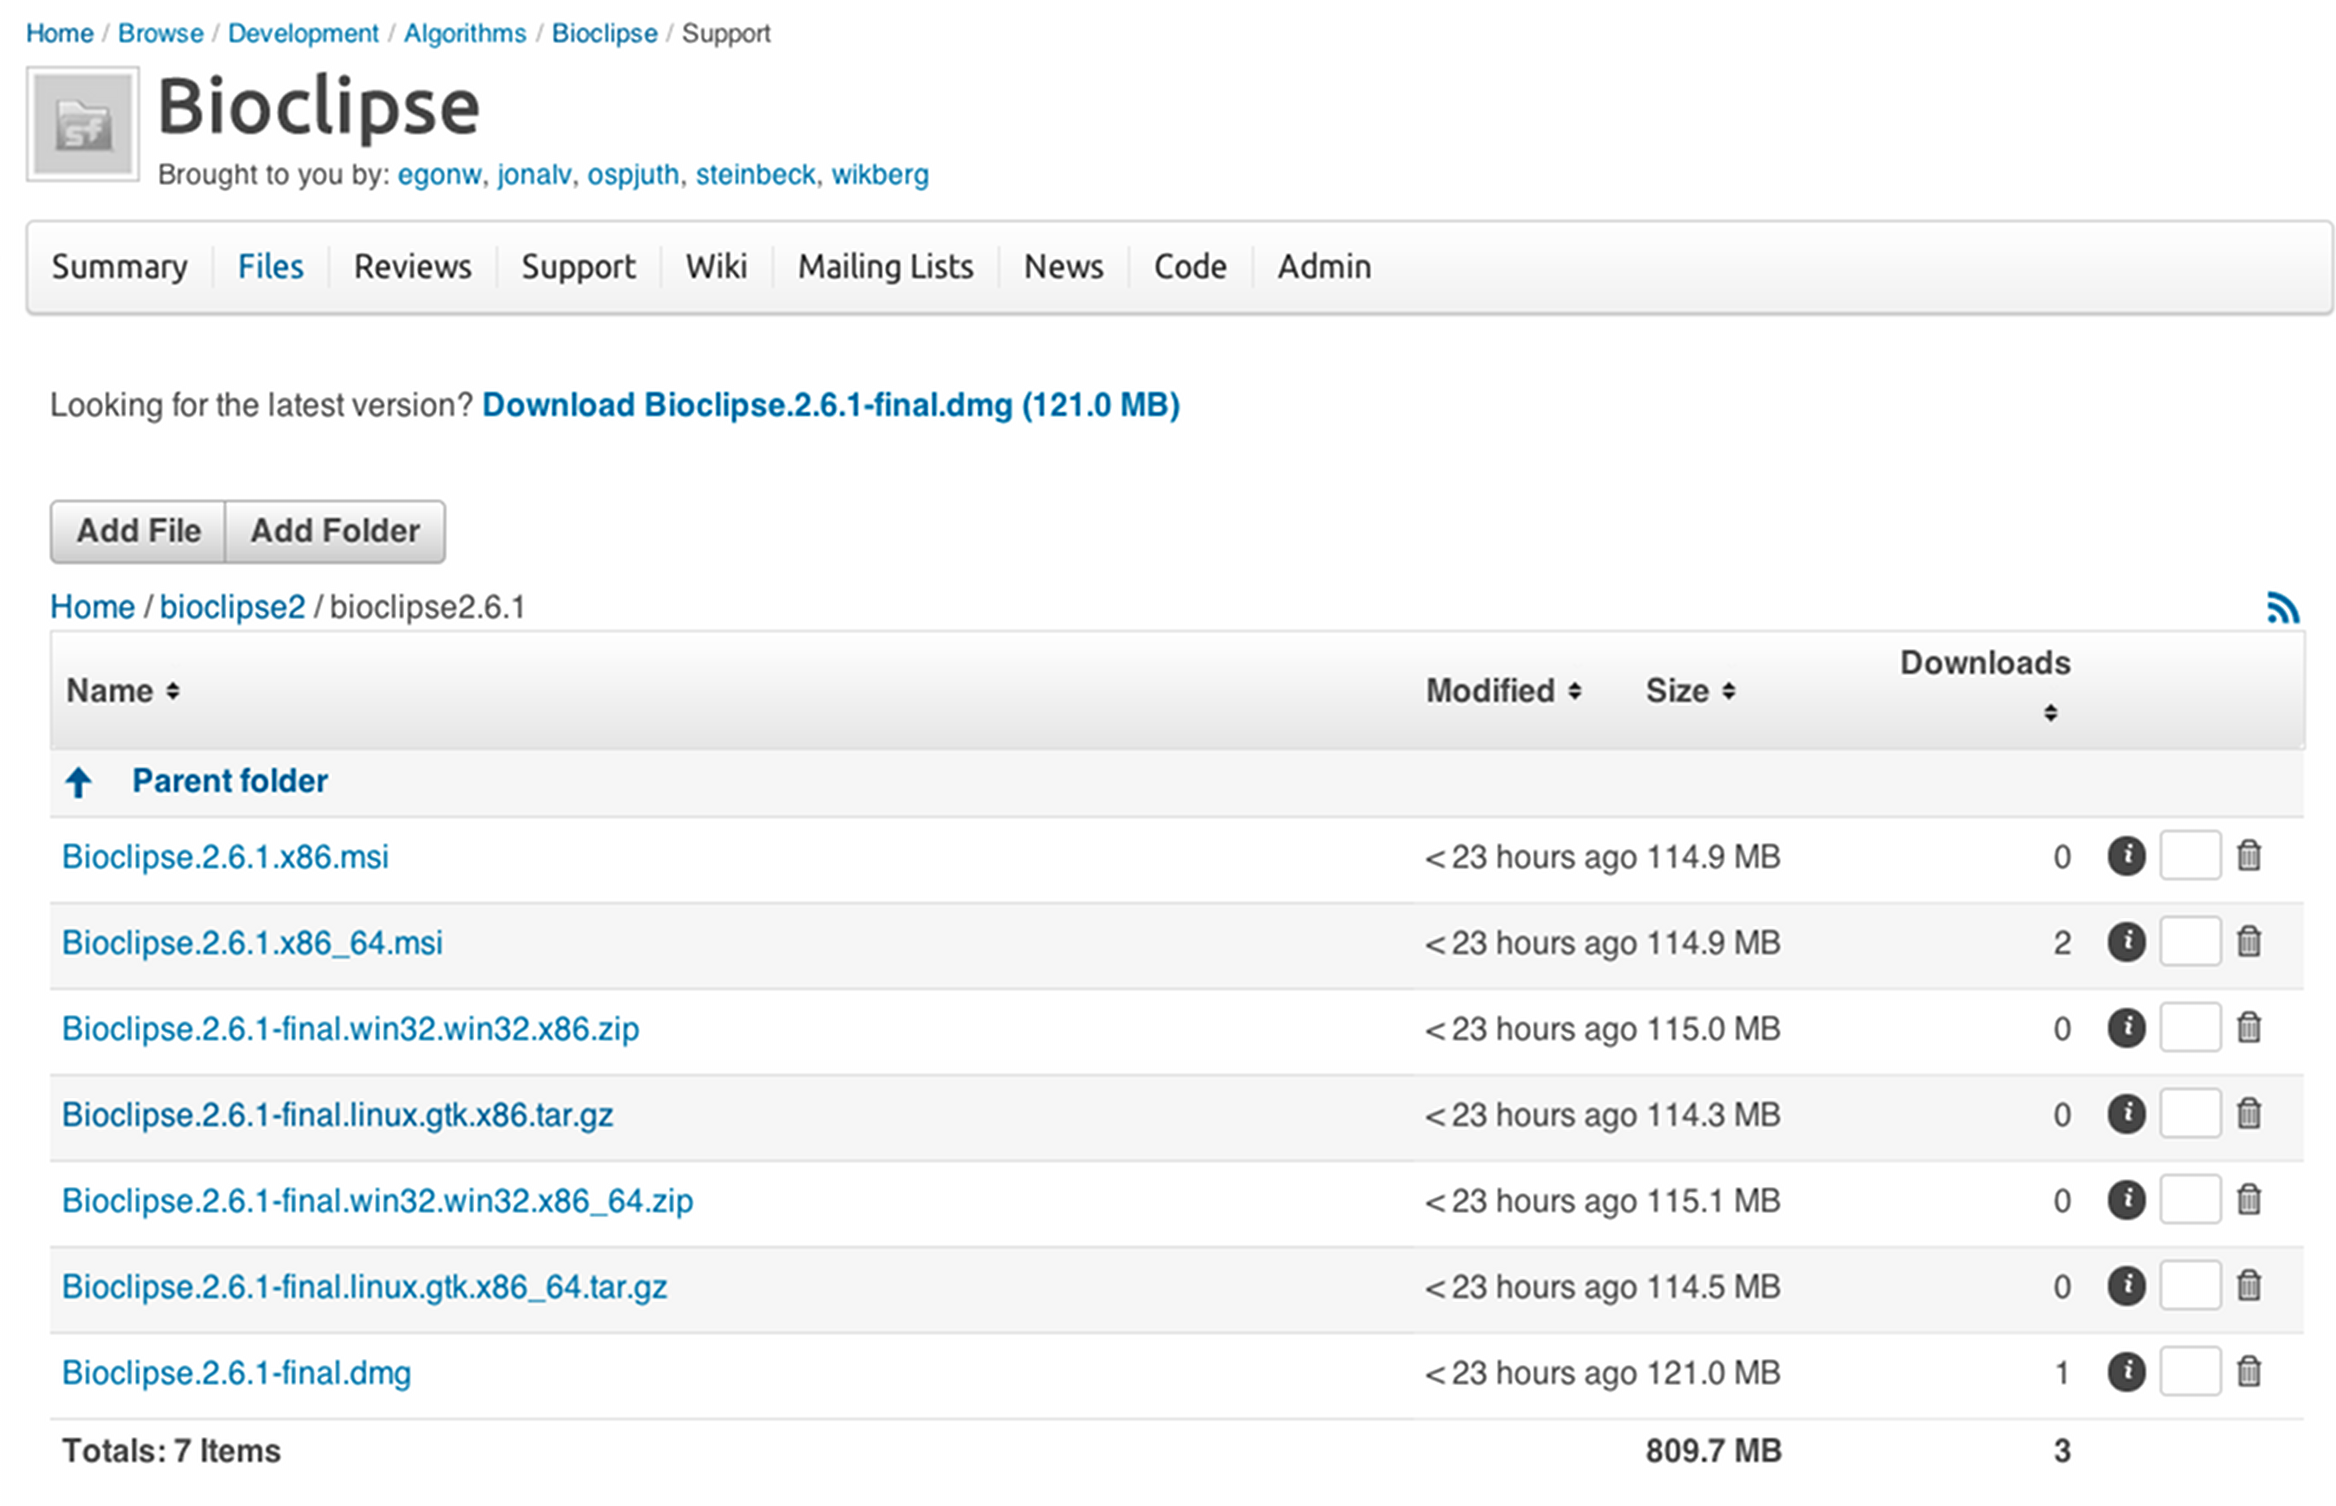
\includegraphics[width=0.95\textwidth]{images/Downloadpage.png}}
\end{center}

\subsubsection{Bioclipse 2.6.2}

The current development version that will lead to the Bioclipse 2.6.2 release
can also be downloaded, and is needed for some of the extensions listed
in this book. For that go to:

\vskip 0.5\baselineskip
{\footnotesize \noindent \url{http://wiki.bioclipse.net/index.php?title=Download}.}


\subsection{Installing}
The installation procedure differs between the operating systems. Bioclipse
needs a Java installation to be present on the computer. To install Java, visit
\url{www.java.com} and follow the instructions. If you are not sure whether or
not you have Java, you can also check that on \url{www.java.com}.

\Needspace{8\baselineskip}
\subsubsection{Windows XP, 7 and 8}
If you downloaded Bioclipse as a \texttt{.zip} file you need to unzip it to a
location where you want it and then start it from the \texttt{Bioclipse.exe}
file. If you downloaded the installation program simply double click the file
to start the installation program which will install Bioclipse on your machine
and add it to the Start menu (on Windows~XP, and Windows~7).
\begin{center}
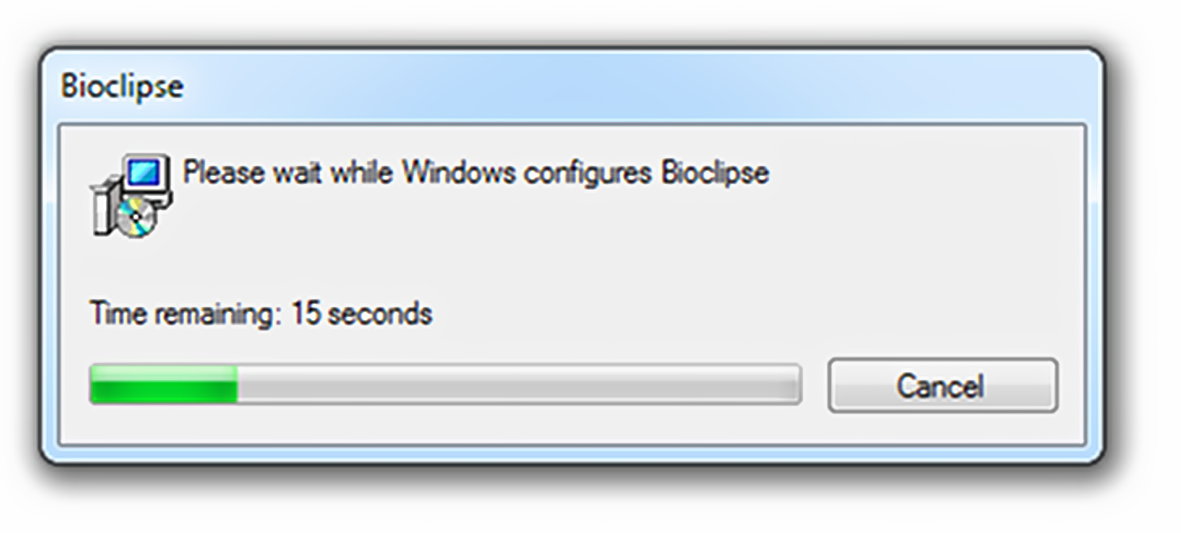
\includegraphics[width=0.8\textwidth]{images/WindowsInstaller.png}
\end{center}
\Needspace{8\baselineskip}
\subsubsection{Mac OS X}
The installation on Mac consists of dragging the \texttt{.app} file to the
Applications folder. You then start Bioclipse from the Applications folder just
like any other program. 
\begin{center}
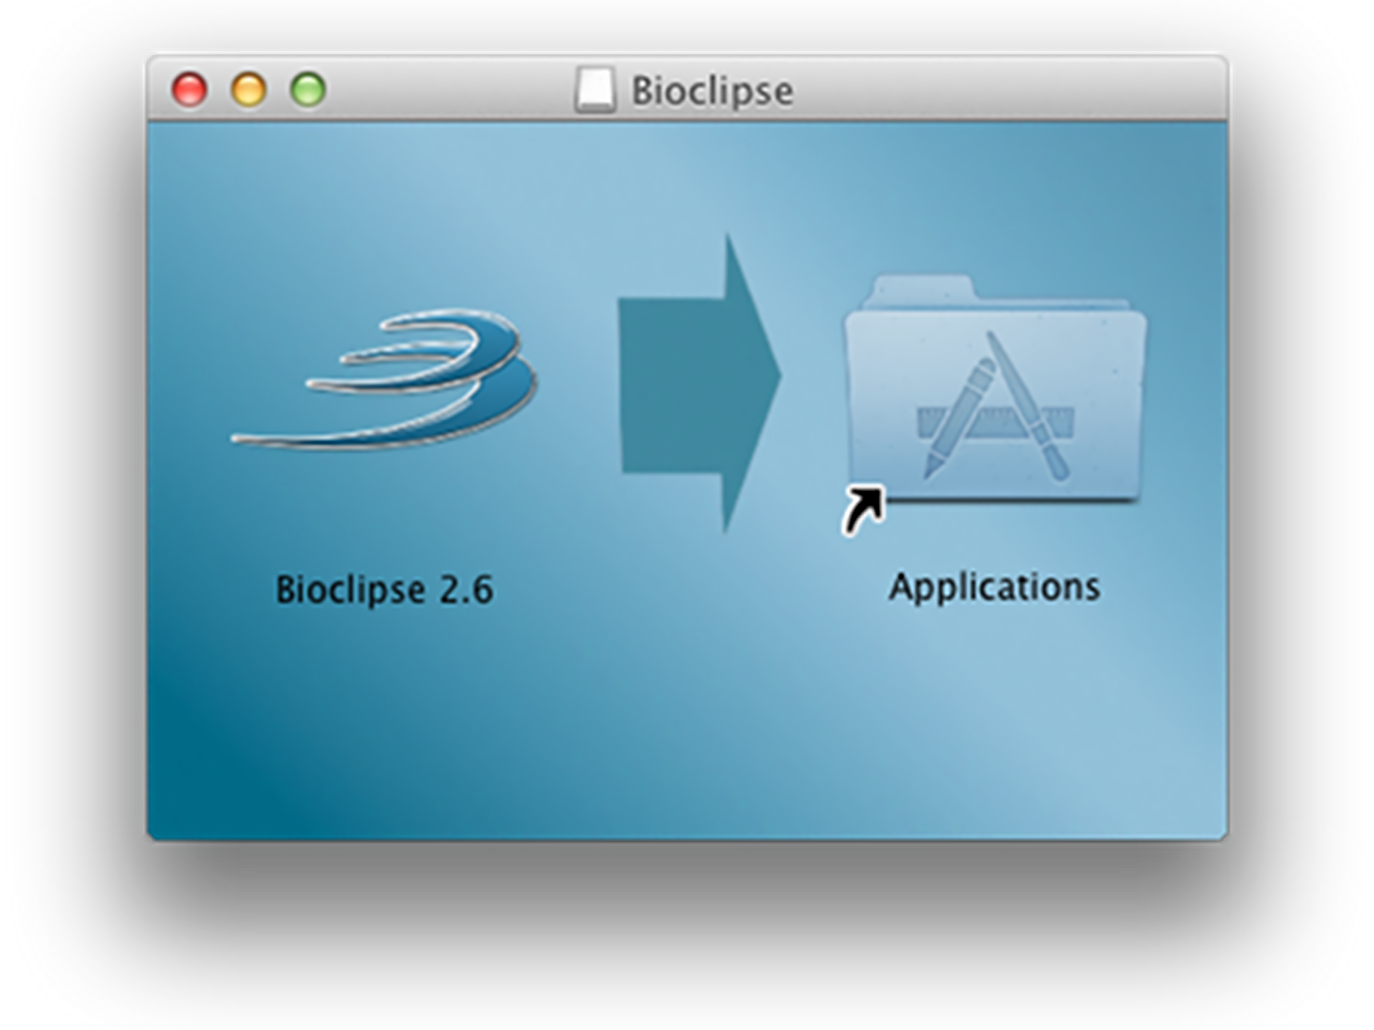
\includegraphics[width=0.7\textwidth]{images/MacInstaller.png}
\end{center}
\subsubsection{Ubuntu Linux}
There is nothing special about the Linux distribution Ubuntu with regards to
Bioclipse and it should work fine with other distributions as well. However we
have tested Ubuntu and show how to get it running on Ubuntu. Hopefully you can
adapt the instructions to your local distribution.
The Linux version of Bioclipse comes packed in a tar.gz file. All you need to
do is to unpack the file to some suitable location and start from there.
Bioclipse uses Java and has been tested with OpenJDK on Ubuntu Linux and Debian
GNU/Linux. 

OpenJDK can be found by searching for `Java' at the Ubuntu software center.
When you have found OpenJDK there, Java can be installed by just a simple
click. The way to install OpenJDK can differ in other distributions of Linux,
but as soon as you have installed OpenJDK Bioclipse should be runnable. When
Java has been properly installed, Bioclipse can be started by double clicking
the file named bioclipse.
\vfill
\begin{center}
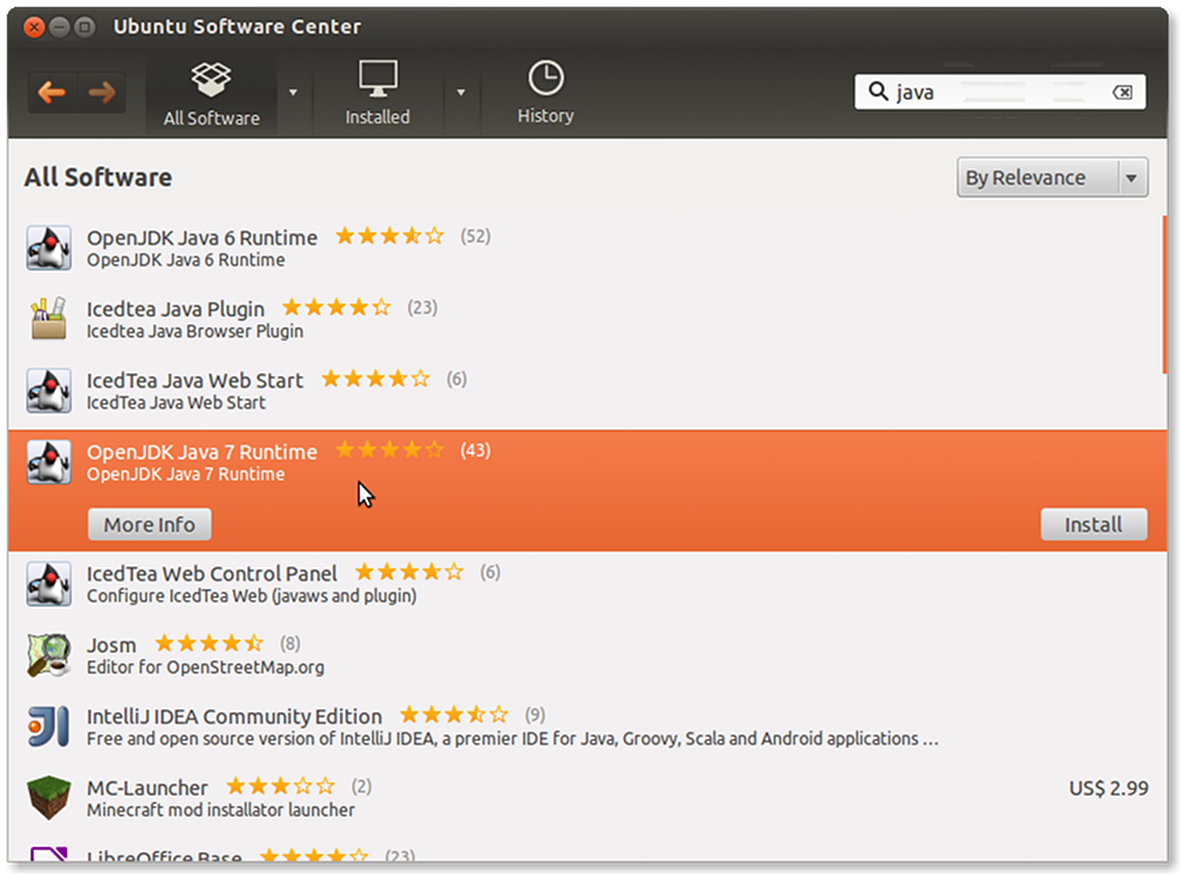
\includegraphics[width=1\textwidth]{images/Java7onUbuntu.png}
\end{center}
\vfill\vfill

\Needspace{17\baselineskip}
\subsection{Starting Bioclipse for the first time}
When you start Bioclipse for the first time a Welcome page is shown.
\begin{center}
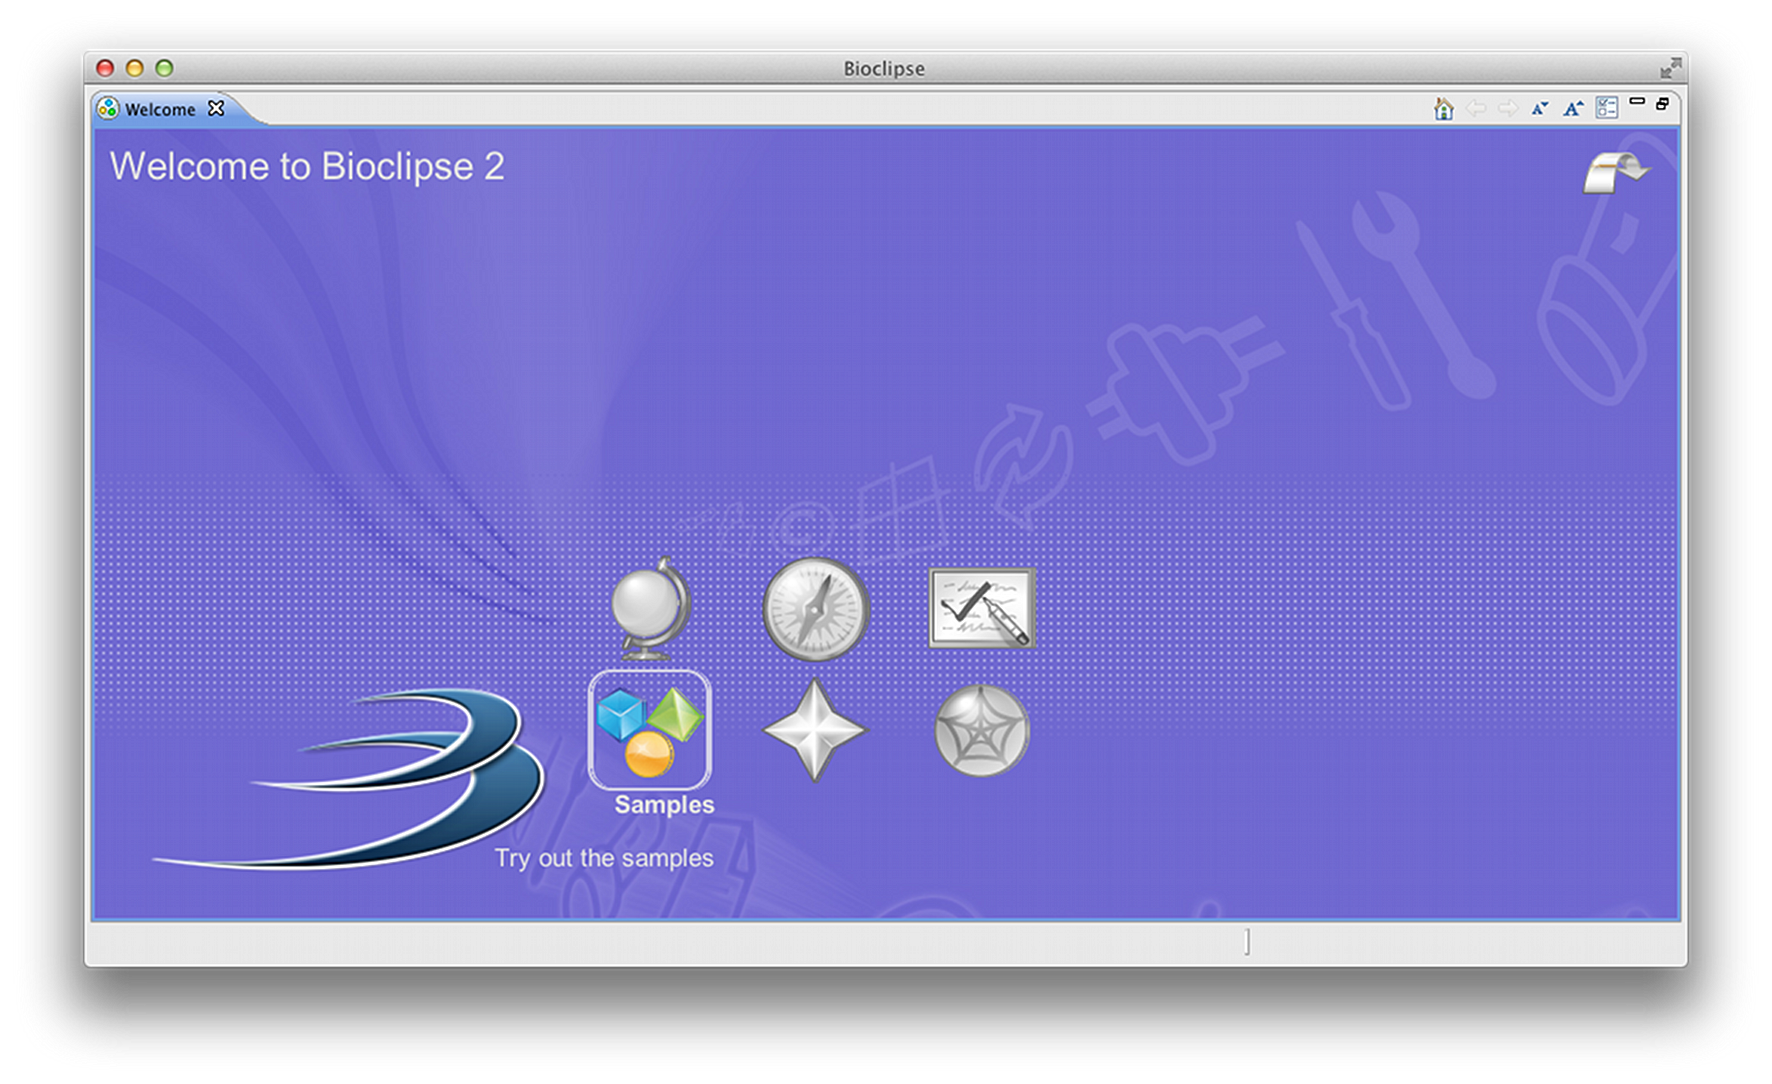
\includegraphics[width=1\textwidth]{images/WelcomePage.png}
\end{center}
Spend some time looking at the various sub pages. Make sure to import the
sample data if you want some data to play with. Just the empty workspace makes
it difficult to test the different parts of Bioclipse.
\begin{center}
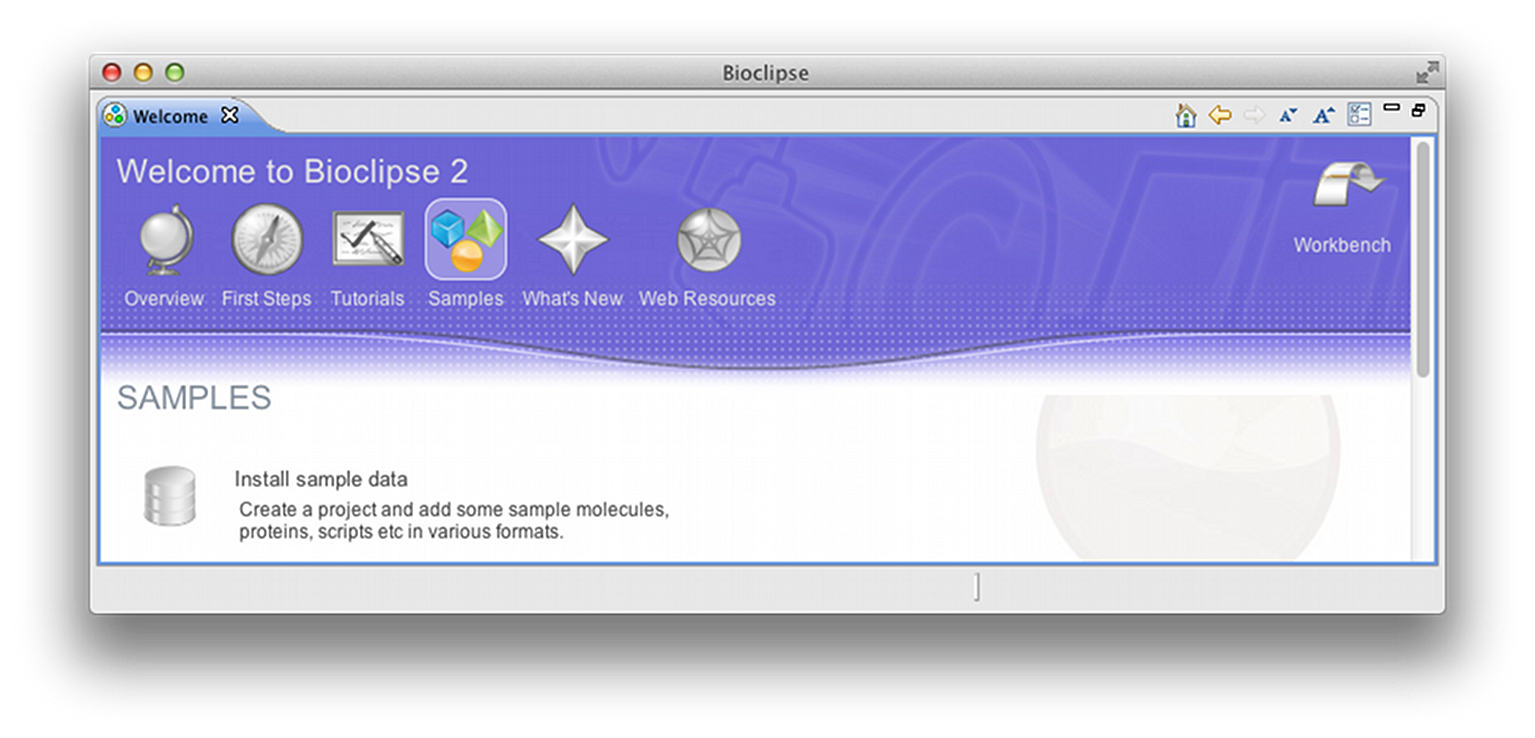
\includegraphics[width=1\textwidth]{images/installSampledata.png}
\end{center}
The arrow in the upper corner brings you to the workbench. If you didn't try
the \texttt{Introductory} \texttt{Bioclipse} \texttt{tutorial} from the Welcome
page it is also reachable from the \texttt{Help} menu by choosing \texttt{Cheat
Sheets} and then selecting the \texttt{Using the Bioclipse Workbench} cheat
sheet. It might be a good idea to spend some time following the instructions in
this cheat sheet before you start exploring Bioclipse on your own.
\begin{center}
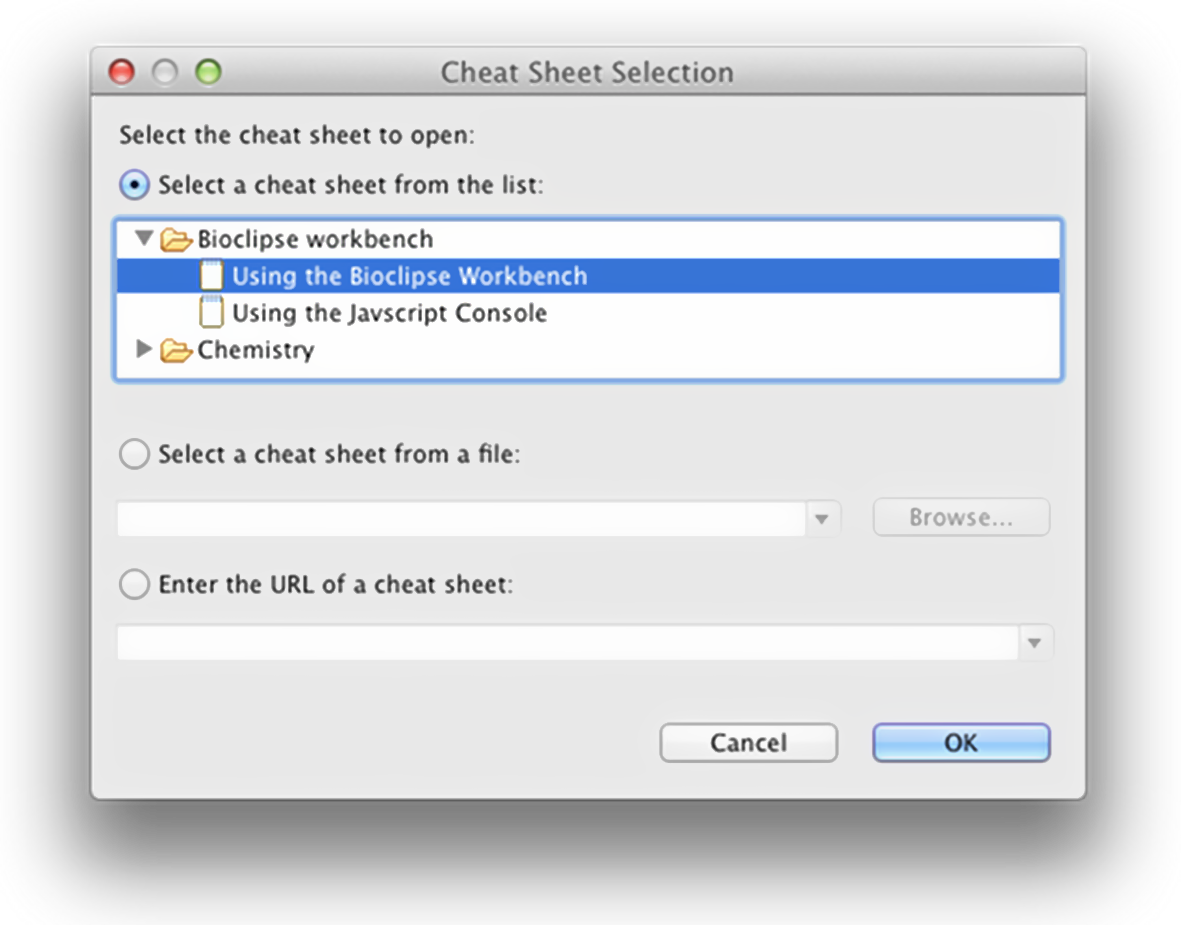
\includegraphics[width=1\textwidth]{images/cheatSheet.png}
\end{center}


\section{Scripting Languages}

Bioclipse supports scripting in three programming languages:
JavaScript\index{JavaScript}, Groovy\index{Groovy}, and Python\index{Python}.
Support for other programming languages is possible, but needs some additional
funding for development. All these languages are enriched with domain
extensions, but it should be noted that the JavaScript support is the
longest existing and the best developed.

\section{Extensions}

Extensions of the scripting language are called \emph{managers}.
These managers introduce domain specific functionality, for
example, in the field of cheminformatics.

Besides managers, Bioclipse also extends the scripting language with a few
basic, helpful commands. For example, to get documentation you can use the
\texttt{man} command, for example, for itself:\index{man}
\begin{Verbatim}
man man
\end{Verbatim}
BTW, help is a synonym:\index{help}
\begin{Verbatim}
help man
\end{Verbatim}
Another interesting command is the doi command which opens a web page with a
paper describing the (tool behind the) functionality of a manager. For example,
to get help for the cdk manager, you type:\index{doi}

\begin{Verbatim}
doi cdk
\end{Verbatim}

\subsection{Updating and installing new features} 
Bioclipse is a highly customizable piece of software. New features and new
versions of features can be installed as needed in your Bioclipse
installation.

When Bioclipse starts, it checks the update site for new versions of what is
already installed. If new versions are found, you are given the option to
download them. If you choose to do so, the new versions will be downloaded.
Once this is done, Bioclipse must be restarted to allow the new features to be
used.

Bioclipse ships with, among other things, components for handling molecules but
more advanced things like, for example, OpenTox support must be installed
separately. To do this click \texttt{Install} in the top menu and then choose
\texttt{New}~\texttt{Feature}\ldots\ This brings up a dialog showing all
features available for installation. By clicking the check box named
\texttt{Show} \texttt{installed} you can also see what features are already
installed in your workbench.

\begin{center}
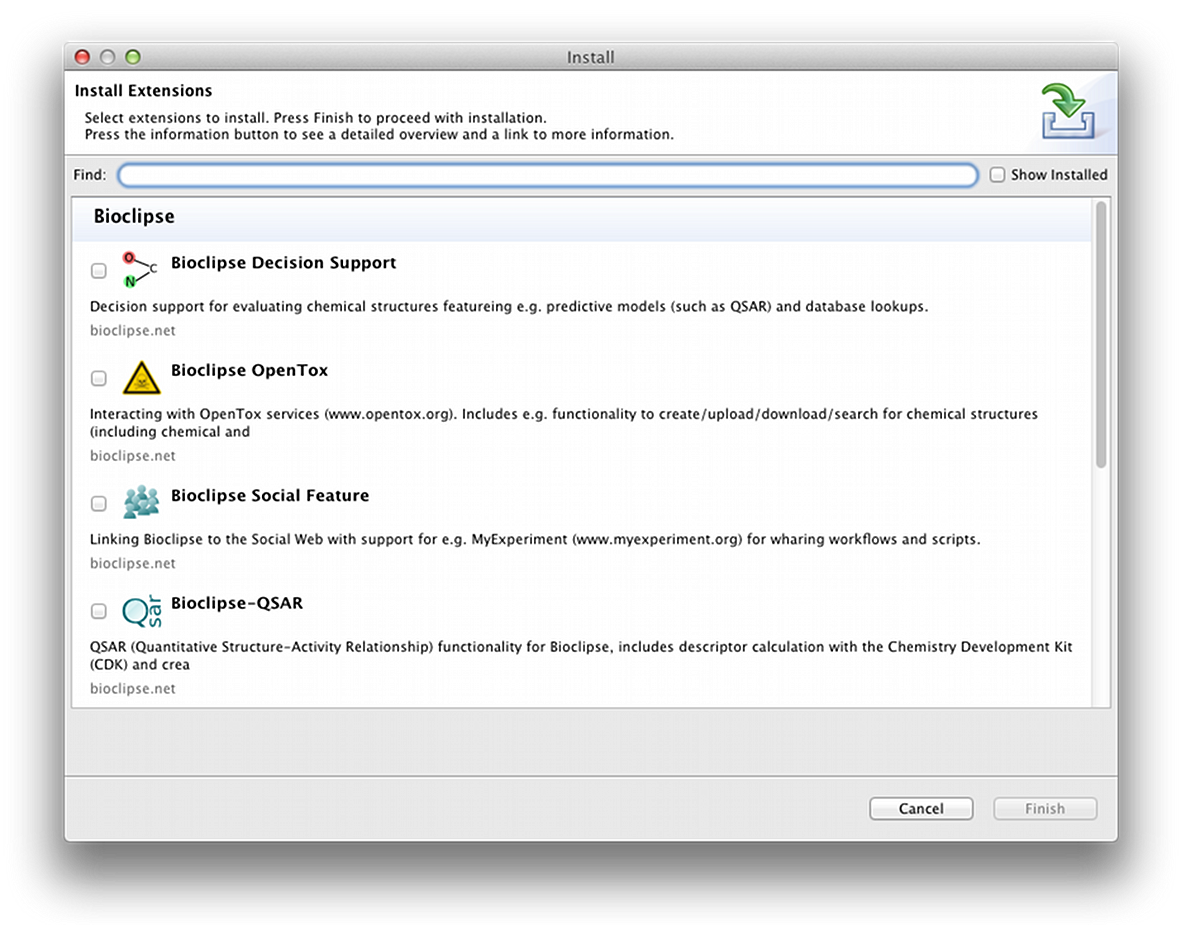
\includegraphics[width=0.95\textwidth]{images/installFeatures.png}
\end{center}

Select what you want to install, accept the licenses and wait while Bioclipse
restarts with the new features.

\subsubsection{Installing beta extensions}

However, the update site providing the features above, does not normally have
newer extensions, particularly not those available for Bioclipse 2.6.2 available
from the nightly build service. This section hopefully provides enough details
to allow the readers to install other Bioclipse extensions too.

The first step is to enable the \texttt{Advanced Mode}; that is, unless you are
advanced, forget about this. Fortunately, the fact that you have not given up on
reading my blog yet is a good indicated you are advanced. Go to the
\texttt{Window} menu and select \texttt{Preferences} and enable the \texttt{Advanced Mode}
in the dialog, as shown here:

\begin{center}
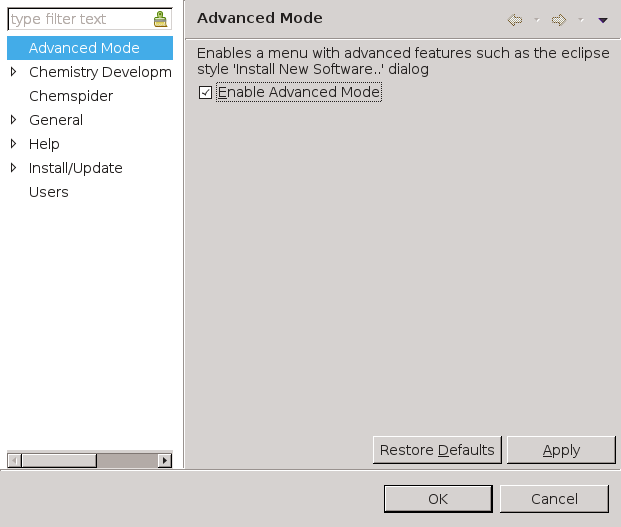
\includegraphics[width=0.65\textwidth]{images/bcAdvancedMode.png}
\end{center}

When done, click Apply and close the dialog with OK. 

The advanced mode you just enablded, basically allows you to add any arbitrary
update sites, like update sites available from the Uppsala build system.
To add new update sites, use this new option select in the \texttt{Install} menu
the \texttt{Software from update site...} option:

\begin{center}
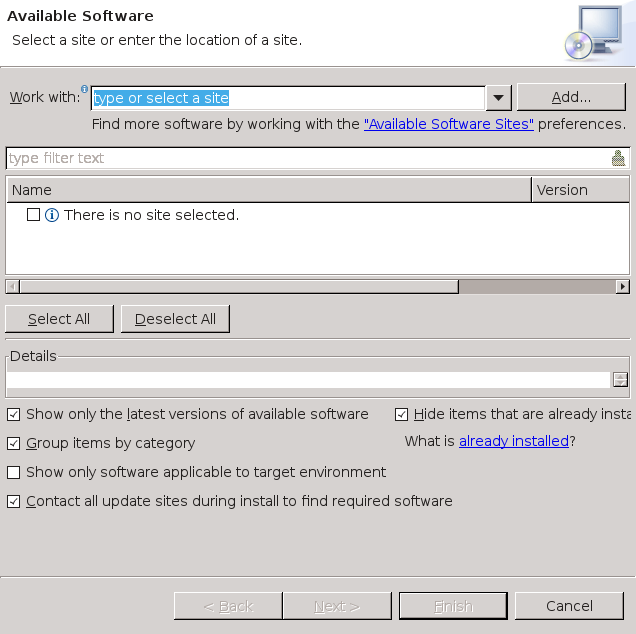
\includegraphics[width=0.65\textwidth]{images/bcUpdateSites.png}
\end{center}

By clicking the Add button, you go this dialog where you should enter the update
site information:

\begin{center}
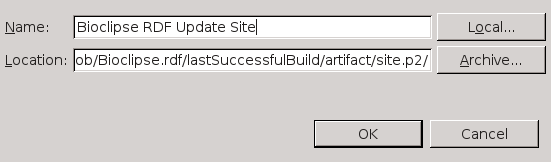
\includegraphics[width=0.65\textwidth]{images/bcUpdateSites1.png}
\end{center}

You need to repeat these steps for each update site you like to use, and you
will likely repeatedly see this dialog, though the content may change from time to
time (the later sections in the book mention various update sites). The
information you need to enter is (the name is not too important and can be something
else that makes sense to you):

\begin{enumerate}
\item Name: Bioclipse RDF Update Site
\item Location: \url{http://pele.farmbio.uu.se/jenkins/job/Bioclipse.rdf/lastSuccessfulBuild/artifact/site.p2/}
\end{enumerate}

After clicking OK in the above dialog, you will return to the Available Software dialog (shown earlier).
The Available Software dialog will now show a list of features available from the just added update site.
If you select your new update site, the dialog will show you the features that you can install from
this update site:

\begin{center}
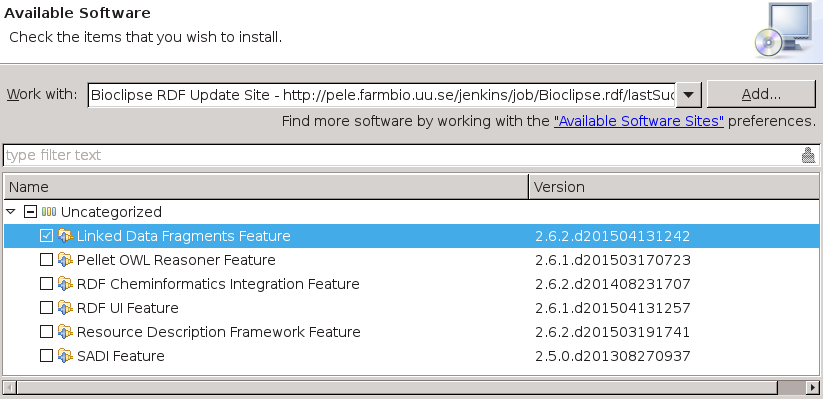
\includegraphics[width=0.65\textwidth]{images/bcUpdateSites2.png}
\end{center}

\section{Domain Objects}

Script extensions are not enough to do bio- and cheminformatics. If extension
cannot exchange data with each other, it will not really be useful. Embedding
of the extensions in the same scripting language is the first step, but
these extensions also need a common data model. This is what the domain objects are
for\index{domain object}.

For example, Bioclipse knows the following domain objects used in the sciences:

\vspace{0.25cm}
\begin{tabular}{ l l }
  IMolecule\index{IMolecule}\index{molecule} & a chemical structure \\
  IProtein\index{IProtein}\index{protein} & a protein sequence \\
  IProteinCrystal\index{IProteinCrystal} & a protein crystal structure \\
\end{tabular}
\vspace{0.25cm}

Furthermore, a further set of more general objects are defined:

\vspace{0.25cm}
\begin{tabular}{ l l }
  IRDFStore\index{IRDFStore}\index{RDF} & a triple store \\
\end{tabular}
\vspace{0.25cm}

\printbibliography[heading=subbibliography]
\end{refsection}




\chapter{Core functionality}
\begin{refsection}

The core functionality of Bioclipse is provided by a set of managers which are part
of the default Bioclipse distribution. This includes the \textit{bioclipse},
\textit{js}, \textit{ui}, and \textit{gist} managers.

\section{The bioclipse manager}\index{manager!bioclipse}\index{bioclipse}

One core manager is the \emph{bioclipse} manager. 

\subsection{Project and file management}
The \emph{bioclipse} manager has, for example,
functionality to convert Eclipse-style paths, based on projects to full
operating system-style paths, which you may need in the scripting language. For
example, given a project in Bioclipse called ``WikiPathways'' with a folder
called ``data'', I can get the full path with:\index{fullPath}
\begin{Verbatim}
fullPath = bioclipse.fullPath(
  "/WikiPathways/data/" + species + "/"
)
\end{Verbatim}
This full path I can then use with, for example, the Java
\emph{File} class from JavaScript and Groovy. For example,
I am using Groovy in this set up:
\begin{Verbatim}
dataMap = bioclipse.fullPath(
  "/WikiPathways/data/" + species + "/"
);
gpmlFiles = new File(dataMap).listFiles()
\end{Verbatim}

\subsection{Runtime environment}
Furthermore, the bioclipse manager has functionality to get some information
about the running Bioclipse. You can get the version with:\index{version}
\begin{Verbatim}
bioclipse.version()
\end{Verbatim}
And get the location of where the log file is
found:\index{logfileLocation}
\begin{Verbatim}
bioclipse.logfileLocation()
\end{Verbatim}
And provide the locations of a few Bioclipse websites\index{Bioclipse wiki}\index{Planet Bioclipse}\index{Bioclipse Bug Tracker}:
\begin{Verbatim}
bioclipse.wiki()
bioclipse.planet()
bioclipse.bugTracker()
\end{Verbatim}

It can be used to test if there is an Internet
connection:\index{isOnline}
\begin{Verbatim}
bioclipse.isOnline()
\end{Verbatim}
But it can also fail if Bioclipse does not have active Internet
access:\index{assumeOnline}
\begin{Verbatim}
bioclipse.assumeOnline()
\end{Verbatim}

The manager can be used to validate some of these assumptions. For example, it
can be used to test which Bioclipse version we are running, or make an
assertion on the minimally required version:\index{requireVersion}
\begin{Verbatim}
bioclipse.requireVersion("2.6.1")
\end{Verbatim}
The bioclipse manager is also the place to look if you would like to download a
web page, such as the front page of the Dutch newspaper "De
Volkskrant":\index{download!webpage}
\begin{Verbatim}
bioclipse.download("http://www.vk.nl/")
\end{Verbatim}


\section{The gist manager}\index{manager!gist}\index{gist}

The gist manager is used for downloading gists. A gist is a simple way to share
small texts on GitHub\index{GitHub}, such as Bioclipse scripts and get verson
control on them. For more information see \url{https://gist.github.com/}.

Originally, a gist was a single file, but that is past history. The manager
followed this change and will now download all files from a
gist:\index{download!gist}

\begin{Verbatim}
gist.download(6282642)
\end{Verbatim}

\section{The js manager}\index{manager!js}\index{js}
The \emph{js} manager is one specific for the JavaScript environment. It has a few
commands that allow you to interact with the console, for example. To clear the
content and write something in the JavaScript console you can use:
\begin{Verbatim}
js.clear()
js.say("Hello world!")
\end{Verbatim}

\section{The ui manager}\index{manager!ui}\index{ui}

Another core manager is the \emph{ui} manager. It has user interface related
functionality. For example, we can use it to test if a file is available from
the Bioclipse workspace:\index{fileExists}

\begin{Verbatim}
knowledgebase = "/WikiPathways/chebi.owl";
if (ui.fileExists(knowledgebase)) {
}
\end{Verbatim}

If we combine this with three further commands, we have a means to modify the
content of files:\index{append}\index{remove}\index{newFile}
\begin{Verbatim}
outFilename = "/eNanoMapper/affinity.ttl"
if (ui.fileExists(outFilename)) {
  ui.remove(outFilename)
  ui.newFile(outFilename)
}
ui.append(outFilename, rdf.asTurtle(store))
\end{Verbatim}

\subsection{An Interactive User Interface}

Importantly, this manager also takes care of interaction with the Bioclipse
user interface itself. For example, we can use it to open editors for
particular blobs of data:\index{open}

\begin{Verbatim}
ui.open(cdk.fromSMILES("c1=cc=cc=c1"))
\end{Verbatim}

And it can show a particular file in the Bioclipse Navigator:\index{Bioclipse Navigator}\index{revealAndSelect}
\begin{Verbatim}
ui.revealAndSelect("/eNanoMapper/affinity.ttl")
\end{Verbatim}

\section{The xml manager}\index{manager!xml}\index{xml}\index{XML}

There is also an \emph{xml} manager to work with XML files. For example, we can test if the
file is well-formed:
\begin{Verbatim}
xml.isWellFormed("/Google/solubility.rdf")
\end{Verbatim}

And list all the XML namespaces in that file:
\begin{Verbatim}
xml.listNamespaces("/Google/solubility.rdf")
\end{Verbatim}

Validation is also possible, using the information in the XML file itself:
\begin{Verbatim}
xml.validate("/Google/solubility.rdf")
\end{Verbatim}
This has the disadvantages that this information must be provided and that you likely
need internet access. However, you can also validate against a file you provide:
\begin{Verbatim}
xml.validateAgainstRelaxNG(
  "/Google/solubility.rdf", relaxNGSchemaFile
)
xml.validateAgainstSchematron(
  "/Google/solubility.rdf", schematronFile
)
xml.validateAgainstXMLSchema(
  "/Google/solubility.rdf", xmlSchemaFile
)
\end{Verbatim}


%\printbibliography[heading=subbibliography]
\end{refsection}




\chapter{Bioinformatics}
\begin{refsection}

\section{The biojava manager}\index{manager!biojava}\index{biojava}

\begin{tabular}{ll}
\textbf{Feature} & Bioinformatics Feature \\
\textbf{Update site} & default \\
\end{tabular}\\

\noindent
BioJava is a library oriented at \textsc{dna}, \textsc{rna}, and protein
sequences\cite{holland2008biojava,prlic2012biojava}.\index{BioJava} With this
manager we can create data models for sequences, such as a \textsc{dna}
sequence from \textsc{fasta} string:\index{DNAsFromString}

\begin{Verbatim}
dna = biojava.DNAsFromString("> foo\nGCAT")
\end{Verbatim}
Or from just a sequence string, with or without a
name:\index{DNAfromPlainSequence}

\begin{Verbatim}
dna = biojava.DNAfromPlainSequence("GCAT")
dna = biojava.DNAfromPlainSequence(
  "GCAT", "dummy sequence"
)
\end{Verbatim}
With two additional methods, we now have a pipeline to convert
\textsc{dna}\index{DNA} into \textsc{rna}\index{RNA}, and \textsc{rna} into a
protein\index{protein} sequence:\index{transcriptionOf}\index{translationOf}

\begin{Verbatim}
dna = biojava.DNAfromPlainSequence("GCATATGAA")
rna = biojava.transcriptionOf(dna)
prot = biojava.translationOf(rna)
\end{Verbatim}

\section{The bridgedb manager}\index{manager!bridgedb}\index{bridgedb}

\begin{tabular}{ll}
\textbf{Feature} & Bioclipse BridgeDb \\
\textbf{Update site} & \url{http://pele.farmbio.uu.se/jenkins/job/bioclipse.bridgedb/lastSuccessfulBuild/artifact/buckminster.output/net.bioclipse.bridgedb_site_1.0.0-eclipse.feature/site.p2/} \\
\end{tabular} \\

\noindent
BridgeDb is a platform for identifier mapping~\cite{van2010bridgedb}. The
Bioclipse manager makes its functionality available.

At the core, BridgeDb is a framework, but the project also provides actual
identifier mapping databases. And, of course, when you want to use \textsc{id}
mapping functionality, you first need to load such a database. The plugin is
written such that \textsc{id} mapping databases can be downloaded as Bioclipse
plugins, and the extension mechanism allows the manager to list which mapping
databases are available:\index{listIDMapperProviders}
\begin{Verbatim}
dbList = bridgedb.listIDMapperProviders()
\end{Verbatim}
And then the available mapping databases can be loaded, for example, the first
in this example:\index{getIDMapper}

\begin{Verbatim}
mbMapper = bridgedb.getIDMapper(dbList.get(0))
\end{Verbatim}
Mind you, BridgeDb has separate identifier mapping databases for genes and
proteins and for metabolites.

And once we have a mapper then we can start converting
identifiers:\index{xref}\index{map}

\begin{Verbatim}
casXref = bridgedb.xref("50-00-0", "Ca")
mappings = bridgedb.map(mbMapper, casXref)
\end{Verbatim}

\printbibliography[heading=subbibliography]
\end{refsection}




\chapter{Cheminformatics}
\begin{refsection}


\section{The cdk manager}\index{manager!cdk}\index{cdk}

\begin{tabular}{ll}
\textbf{Feature} & Bioclipse Chemoinformatics \\
\textbf{Update site} & default \\
\end{tabular} \\

\noindent
Basic cheminformatics in Bioclipse is mainly handled by the Chemistry
Development Kit\index{Chemistry Development Kit}\index{CDK}
(\textsc{cdk})~\cite{Steinbeck2003,Steinbeck2006} and for this there is the
\emph{cdk} manager.

The cdk manager is one with many features. One is to validate
\textsc{CAS} registry numbers, identifiers used by the Chemical Abstract
Services:\index{CAS registry number}

\begin{Verbatim}
cdk.isValidCAS("50-00-0")
\end{Verbatim}

But let's go to the more interesting functionality around chemical graphs. For
example, let's see how we can create molecular structures from a SMILES
string:\index{SMILES}\index{fromSMILES}

\begin{Verbatim}
mol = cdk.fromSMILES("COC")
\end{Verbatim}
Normally, structure diagrams are generated without explicit hydrogens. But we
can easily add them:\index{hydrogens}\index{addExplicitHydrogens}

\begin{Verbatim}
cdk.addExplicitHydrogens(mol)
\end{Verbatim}
We can then calculate a number of properties, including the molecular
mass\index{molecular mass}, total formal charge\index{charge}, and molecular
formula\index{molecular
formula}:\index{calculateMass}\index{totalFormalCharge}\index{molecularFormula}

\begin{Verbatim}
cdk.calculateMass(mol)
cdk.totalFormalCharge(mol)
cdk.molecularFormula(mol)
\end{Verbatim}
Additionally, we can also inspect some of in the information present in the
model:\index{has2d}\index{has3d}\index{isConnected}

\begin{Verbatim}
cdk.has2d(mol)
cdk.has3d(mol)
cdk.isConnected(mol)
\end{Verbatim}
The cdk manager is also central to file support. Before we load it, we may want
to just check the file format\index{file format}:\index{determineFormat}

\begin{Verbatim}
cdk.determineFormat(
  "/ACS Drug Disclosures/AZD5423.cml"
)
\end{Verbatim}
However, this information is not needed when loading files:\index{loadMolecule}

\begin{Verbatim}
mol = cdk.loadMolecule(
  "/ACS Drug Disclosures/AZD5423.cml"
)
\end{Verbatim}
Saving is quite similar, and there are two methods for the two main formats:

\begin{Verbatim}
cdk.saveCML(mol, "/Test/mol.cml")
cdk.saveMDLMolfile(mol, "/Test/mol.mol")
\end{Verbatim}

\section{The cdx manager}\index{manager!cdx}\index{cdx}


\begin{tabular}{ll}
\textbf{Feature} & Bioclipse CDK Feature \\
\textbf{Update site} & \url{http://pele.farmbio.uu.se/jenkins/job/Bioclipse.chemoinformatics/lastSuccessfulBuild/artifact/buckminster.output/net.bioclipse.chemoinformatics_site_0.0.1-eclipse.feature/site.p2/} \\
\end{tabular} \\

\noindent
The \texttt{cdx} manager is also based on the \textsc{cdk} and exposes
functionality more oriented at \textsc{cdk} developers. For example, we can
create a String representation of the full data model for debugging
purposes:\index{debug}

\begin{Verbatim}
cdx.debug(mol)
\end{Verbatim}
Or we can see the details of the differences between two data
models:\index{diff}

\begin{Verbatim}
cdx.diff(
  cdk.fromSMILES("CC"),
  cdk.fromSMILES("CCC")
)
\end{Verbatim}
And we can list the exact atom types for the atoms in a
molecule:\index{perceiveCDKAtomTypes}\index{atom type}

\begin{Verbatim}
cdx.perceiveCDKAtomTypes(mol)
\end{Verbatim}

\section{The inchi manager}\index{manager!inchi}\index{inchi}

\begin{tabular}{ll}
\textbf{Feature} & Bioclipse Chemoinformatics \\
\textbf{Update site} & default \\
\end{tabular} \\

\noindent
The \texttt{inchi} manager makes functionality from the InChI
standard\index{InChI} available~\cite{heller2013inchi,spjuth2013applications}.
The InChI library is not available as a Java library, but is included as a
binary for a selection of platforms and operating systems. This means that we
cannot assume the InChI functionality is always available in Bioclipse.
Furthermore, we need to load the library:

\begin{Verbatim}
inchi.load()
inchi.isLoaded()
\end{Verbatim}
But when that has succeeded, we can start minting InChIs:\index{generate!InChI}

\begin{Verbatim}
anInChI = inchi.generate(
  opsin.parseIUPACName("methane")
)
\end{Verbatim}
The returned value is a class called InChI and we can get both the full InChI
as well as the InChIKey from it:\index{InChIKey}

\begin{Verbatim}
fullInChI = anInChI.getValue()
InChIKey = anInChI.getKey()
\end{Verbatim}

\section{The opsin manager}\index{manager!opsin}\index{opsin}

\begin{tabular}{ll}
\textbf{Feature} & Bioclipse Chemoinformatics \\
\textbf{Update site} & default \\
\end{tabular} \\

\noindent
The opsin manager makes functionality from the \textsc{opsin}\index{OPSIN}
available: convert \textsc{iupac}\index{IUPAC name} names to chemical
structures~\cite{lowe2011chemical}.

\begin{Verbatim}
mol = opsin.parseIUPACName(
  "Ethyl [(1R,3aR,4aR,6R,8aR,9S,9aS)-9-" +
  "{(E)-2-[5-(3-fluorophenyl)-2-pyridinyl]vinyl}-" +
  "1-methyl-3-oxododecahydronaphtho[2,3-c]furan-" +
  "6-yl]carbamate"
)
\end{Verbatim}

\printbibliography[heading=subbibliography]
\end{refsection}






\chapter{Semantic Web}
\begin{refsection}

Semantic Web technologies are the new glue to link different data sources. Bioclipse
provides support for several of the technologies, including general
Resource Description Format (RDF) support\index{Resource Description Format}\index{RDF},
the SPARQL query language\index{SPARQL}, and the Web Ontology Langauge
(OWL)\index{OWL}\index{Web Ontology Language}. This chapter outlines how these
technologies can be used in Bioclipse.

\section{The rdf manager}\index{manager!rdf}\index{rdf}

\begin{tabular}{ll}
\textbf{Feature} & Resource Description Framework Feature \\
\textbf{Update site} & default \\
\end{tabular} \\

\noindent
The \texttt{rdf} manager can be used to handle Resource Description Framework
(\textsc{rdf}) data~\cite{willighagen2011linking}. The basic unit of
information in \textsc{rdf} is a triple and these triples are stored in a
\emph{triple store}. A file based store can be created with this
code:\index{createStore}

\begin{Verbatim}
base = rdf.createStore("/tmp/chebiowl")
\end{Verbatim}
Here, the path is a full operating system-style path, and this one works only
on Unix/Linux/BSD systems.

As soon as you have a store, you can start adding triples to it. For example,
when they come from a file, you may want to do something like
this:\index{importFile}

\begin{Verbatim}
knowledgebase = "/WikiPathways/chebi.owl";
kbFormat = "RDF/XML";
base = rdf.createStore("/tmp/chebiowl")
rdf.importFile(base, knowledgebase, kbFormat);
\end{Verbatim}
If the amount of data is limited, you can also create an
in-memory model:\index{createInMemoryStore}

\begin{Verbatim}
knowledgebase = rdf.createInMemoryStore();
\end{Verbatim}
This can be used to create triples from data you are
processing:\index{addObjectProperty}\index{addDataProperty}
\index{object property}\index{data property}

\begin{Verbatim}
rdf.addObjectProperty(knowledgebase,
  "http://linkedchemistry.info/chembl/molecule/m443",
  "http://www.w3.org/2000/01/rdf-schema#subClassOf",
  "http://semanticscience.org/resource/CHEMINF_000000"
)
rdf.addDataProperty(knowledgebase,
  "http://linkedchemistry.info/chembl/molecule/m443",
  "http://www.w3.org/2000/01/rdf-schema#label",
  "CHEMBL268854"
)
\end{Verbatim}

You can get the number of triples held in the store with the size
method:\index{size}

\begin{Verbatim}
rdf.size(knowledgebase);
\end{Verbatim}

And the collected set of triples can be serialized as Turtle, which
is one of the easier to read serialization formats of RDF triples.
For this, you can use:\index{Turtle}\index{asTurtle}

\begin{Verbatim}
rdf.asTurtle(knowledgebase);
\end{Verbatim}


\section{The isbjørn manager}\index{manager!isbjørn}\index{isbjørn}

\begin{tabular}{ll}
\textbf{Feature} & Bioclipse Isbjørn \\
\textbf{Update site} & \url{} \\
\end{tabular} \\

\noindent
The \texttt{isbjørn} manager uses the Semantic Web to find information about
chemicals, by taking advantage of the Linked Data approaches.

There are two ways to initiate a search: the first is based on a \textsc{uri}
(Uniform Resource Identifier)\index{URI} for a particular compound, for
example, a ChemSpider\index{ChemSpider} \textsc{uri}:\index{findInfo}

\begin{Verbatim}
knowledgeList = isbjørn.findInfo(
  "http://www.chemspider.com/" +
  "Chemical-Structure.145.rdf#Compound"
)
\end{Verbatim}
But we can also start with a structure:\index{findInfo}

\begin{Verbatim}
knowledgeList = isbjørn.findInfo(
  opsin.parseIUPACName("benzene")
)
\end{Verbatim}
Both methods return a list of \textsc{rdf} stores, one for each data provider.
The results can be saved as a \textsc{html} file with:\index{saveAsHTML}

\begin{Verbatim}
html = isbjørn.saveAsHTML(
  knowledgeList, "/Test/info.html"
)
ui.open(html)
\end{Verbatim}

\section{The owlapi manager}\index{manager!owlapi}\index{owlapi}

\begin{tabular}{ll}
\textbf{Feature} & OWLAPI Feature \\
\textbf{Update site} & \url{http://pele.farmbio.uu.se/jenkins/job/Bioclipse.rdf/lastSuccessfulBuild/artifact/site.p2/} \\
\end{tabular} \\

\noindent
The \texttt{owlapi} manager exposes functionality of the
\textsc{owlapi}\index{OWLAPI} library~\cite{Horridge2011}, to deal with Web
Ontology Languages\index{Web Ontology Languages} (\textsc{owl})\index{OWL}
ontologies. The manager is oriented at ontologies in the Bioclipse workspace.
Thus, loading an ontology works like:\index{load}

\begin{Verbatim}
ontology = owlapi.load(
  "/eNanoMapper/enanomapper.owl", null
);
\end{Verbatim}
The second parameter is a mapper, which can be used to indicate where imported
ontologies can be locally found. For example:\index{addMapping}

\begin{Verbatim}
mapper = null; // initially no mapper
mapper = owlapi.addMapping(mapper,
  "http://purl.bioontology.org/ontology/npo",
  "/eNanoMapper/npo-asserted.owl"
);
mapper = owlapi.addMapping(mapper,
  "http://www.enanomapper.net/ontologies/" + 
  "external/ontology-metadata-slim.owl",
  "/eNanoMapper/ontology-metadata-slim.owl"
)
ontology = owlapi.load(
  "/eNanoMapper/enanomapper.owl", mapper
);
\end{Verbatim}
You can always see what \textsc{iri}s are mapped with:\index{listMappings}

\begin{Verbatim}
owlapi.listMappings(mapper)
\end{Verbatim}
Once you have loaded an ontology, you can list all the imported
ontologies:\index{getImportedOntologies}

\begin{Verbatim}
imported = owlapi.getImportedOntologies(ontology)
for (var i = 0; i < imported.size(); i++) {
  js.say(
    imported.get(i).getOntologyID().getOntologyIRI()
  )
}
\end{Verbatim}
Similarly, you can list all the classes defined by the ontology or imported
ontologies:\index{showClasses}

\begin{Verbatim}
imported = owlapi.getImportedOntologies(ontology)
for (var i = 0; i < imported.size(); i++) {
  js.say(
    owlapi.showClasses(imported.get(i))
  )
}
\end{Verbatim}
Finally, the \textsc{owlapi} also provide functionality to check for profile
violations:\index{checkVioloations}

\begin{Verbatim}
owlapi.checkVioloations(ontology)
\end{Verbatim}

\section{The ldf manager}\index{manager!ldf}\index{ldf}

\begin{tabular}{ll}
\textbf{Feature} & Linked Data Fragments Feature \\
\textbf{Update site} & \url{http://pele.farmbio.uu.se/jenkins/job/Bioclipse.rdf/lastSuccessfulBuild/artifact/site.p2/} \\
\end{tabular} \\

Linked Data Fragments (LDF)\index{Linked Data Fragments} are a novel technology allowing
distributed querying. The LDF software used in Bioclipse provides the functionality
by exposing a \emph{fragment} as a RDF store. That is very fortunate, because it
means we can automatically integrate it with the existing RDF functionality, for example
provided by the \emph{rdf} manager. For example, we can query for and validate CAS
registry numbers in WikiData:

\begin{Verbatim}
wikidataldf = ldf.createStore(
  "http://data.wikidataldf.com/wikidata"
)

identifier = "P231"

sparql = """
PREFIX wd: <http://www.wikidata.org/entity/>

SELECT ?compound ?id WHERE {
  ?compound wd:${identifier}s [ wd:${identifier}v ?id ] .
}
"""
mappings = rdf.sparql(wikidataldf, sparql)

// safe to a file
for (i=1; i<=mappings.rowCount; i++) {
  casNo = mappings.get(i, "id")
  compound = mappings.get(i, "compound")
  if (!cdk.isValidCAS(casNo)) {
    js.say(
      "Compound " + compound + " has an " +
      " invalid CAS registry number: " +
      casNo
    );
  }
}
\end{Verbatim}



\printbibliography[heading=subbibliography]
\end{refsection}






\chapter{Online Service Providers}
\begin{refsection}

\section{The \texttt{biows} manager}\index{manager!biows}\index{biows}

\begin{tabular}{ll}
\textbf{Feature} & Bioinformatics Feature \\
\textbf{Update site} & \url{} \\
\end{tabular} \\

\noindent
The biows manager allows you to retrieve information from biology-related
webservices, including the Uniprot
database:\index{UniProt}\index{queryUniProtKB}:

\begin{Verbatim}
biows.queryUniProtKB("P38398")
\end{Verbatim}
The \textsc{embl} nucleotide sequence database at the \textsc{ebi}:\index{queryEMBL}

\begin{Verbatim}
biows.queryEMBL("M10051")
\end{Verbatim}
And also RefSeq:\index{queryRefseq}\index{RefSeq}

\begin{Verbatim}
biows.queryRefseq("NM_000059")
\end{Verbatim}

\section{The chemspider manager}\index{manager!chemspider}\index{chemspider}

\begin{tabular}{ll}
\textbf{Feature} & Bioclipse Chemoinformatics \\
\textbf{Update site} & \url{} \\
\end{tabular} \\

\noindent
The chemspider manager makes functionality avaiable to interact with the
ChemSpider database\index{ChemSpider}. For example, we can download a structure
with a chemspider identifier number:\index{download!chemspider}

\begin{Verbatim}
chemspider.download(9606)
\end{Verbatim}
You can also use ChemSpider to resolve InChIKeys to entries in the
database:\index{InChIKey}

\begin{Verbatim}
chemspider.resolve("RCINICONZNJXQF-MZXODVADSA-N")
\end{Verbatim}
Some methods require a security token that can be set via the preferences (see
\url{http://www.chemspider.com/AboutServices.aspx}). But when that is done, we
can search specific compounds:\index{exactSearch}

\begin{Verbatim}
chemspider.exactSearch(
  opsin.parseIUPACName("methane")
)
\end{Verbatim}
Similarly, we can also do a similarity search:

\begin{Verbatim}
chemspider.similaritySearch(
  opsin.parseIUPACName(
    "acetyl salicylic acid"
  ), 0.95
)
\end{Verbatim}
And by substructure:

\begin{Verbatim}
chemspider.substructureSearch(
  opsin.parseIUPACName("benzene")
)
\end{Verbatim}

\section{The google manager}\index{manager!google}\index{google}

\begin{tabular}{ll}
\textbf{Feature} & Google Feature \\
\textbf{Update site} & \url{http://pele.farmbio.uu.se/jenkins/job/Bioclipse.ons/lastSuccessfulBuild/artifact/buckminster.output/net.bioclipse.ons_site_1.0.0-eclipse.feature/site.p2/} \\
\end{tabular} \\

Google Drive is an convenient online collaboration tool, though it does
require an account, and the Spreadsheet functionality allows sharing data between
researchers. Bioclipse has functionality to extract data from online Google
Spreadsheets. For this to work, you need to have a password for an app, as
your Google account password cannot be used. This specific, 16 character, password
needs to be manually created using your webbrowser, following this link:
\url{https://security.google.com/settings/security/apppasswords}. Create a new
App password (\textit{"Other (Customized name)"}) and use this password in Bioclipse:

\begin{Verbatim}
google.setUserCredentials(
  "your.account", "16charpassword"
)
\end{Verbatim}

This call will not check the credentials, but set it for later calls to this
manager. For example, it will be used when you list all spreadsheets on your
account:

\begin{Verbatim}
google.listSpreadsheets()
\end{Verbatim}

For a particular spreadsheet you can then list all worksheets:

\begin{Verbatim}
google.listWorksheets(
  "ORCID @ Maastricht University"
)
\end{Verbatim}

And with both the spreadsheet name and one of its worksheets, I can download
this as a \textsc{StringMatrix}:

\begin{Verbatim}
data = google.loadWorksheet(
  "ORCID @ Maastricht University",
  "with works"
)
\end{Verbatim}

Of course, the names need to match a spreadsheet on your Google Drive.

\section{The openphacts manager}\index{manager!openphacts}\index{openphacts}

Open PHACTS\index{Open PHACTS} is a semantic web-based knowledge platform under
development to support drug discovery~\cite{Williams2012}. It provides a
REST-like interface of which some of the methods are exposed by the openphacts
managers. Because it is a semantic web platform, compounds, diseases, proteins,
and pathways are all identified with URIs. Practically, however, we start with
a name, but usign the Open PHACTS ``identity resolution service'' (IRS) we can
convert names into URIs:\index{search!openphacts}

\begin{Verbatim}
cwHits = openphacts.lookUpCompounds("aspirin")
\end{Verbatim}
From the list, we can get a URI with:

\begin{Verbatim}
compoundURI = cwHits.get(0).getURI()
\end{Verbatim}
Another approach to look up a URI for a compound and, as such, find the
compound in the knowledge base, is to start with an IMolecule:

\begin{Verbatim}
compoundURI = openphacts.getURI(
  cdk.fromSMILES("CC(=O)OC1=CC=CC=C1C(=O)O")
)
\end{Verbatim}
If you want to look up information about the search hits, you do:

\begin{Verbatim}
hitsInfo = openphacts.getCompoundsInfo(cwHits)
\end{Verbatim}
Future versions of the manager will likely provide alternative APIs to get
compound information.

Similar compounds can be looked up using the Tanimoto distance measure, and a
similarity cut off of 0.8 by default:

\begin{Verbatim}
similarCompounds = openphacts.findSimilar(
  cdk.fromSMILES("CC(=O)OC1=CC=CC=C1C(=O)O")
)
\end{Verbatim}
If you find that list too long, you can increase the minimal similarity to, for
example, 0.95:

\begin{Verbatim}
similarCompounds = openphacts.findSimilar(
  cdk.fromSMILES("CC(=O)OC1=CC=CC=C1C(=O)O"), 0.95
)
\end{Verbatim}

\section{The opentox manager}\index{manager!opentox}\index{opentox}

\begin{tabular}{ll}
\textbf{Feature} & Bioclipse OpenTox \\
\textbf{Update site} & \url{} \\
\end{tabular} \\

\noindent
OpenTox is a platform for toxicology\index{OpenTox}, allowing for sharing of
data as well as creating and running computational
models~\cite{hardy2010collaborative}. The opentox manager integrates much of its
functionality~\cite{willighagen2011computational}.

There are various methods to list what is available. Some information is
available from a central registration server, e.g.
\url{http://apps.ideaconsult.net:8080/ontology/}:\index{listAlgorithms}\index{listDescriptors}\index{listModels}

\begin{Verbatim}
registry = "http://apps.ideaconsult.net:8080/ontology";
algorithms = opentox.listAlgorithms(registry);
descriptors = opentox.listDescriptors(registry);
models = opentox.listModels(registry);
\end{Verbatim}
Similarly, using a particular OpenTox service, e.g. an
\textsc{ambit}\index{AMBIT} instance at
\url{http://apps.ideaconsult.net:8080/ambit2/}\cite{jeliazkova2011ambit}, we
can list data sets and features
(properties):\index{listDataSets}\index{listFeatures}

\begin{Verbatim}
service = "http://apps.ideaconsult.net:8080/ambit2/";
dataSets = opentox.listDataSets(service);
features = opentox.listFeatures(service);
\end{Verbatim}
Instead of listing, we can also search for various types, such as the ToxTree
models\index{ToxTree}\cite{patlewicz2008evaluation}:

\begin{Verbatim}
models = opentox.searchModels(registry, "ToxTree");
\end{Verbatim}
We can select one of the available models, and then make a prediction for a
compound:
\begin{Verbatim}
toxTreeModel =
  "http://apps.ideaconsult.net:8080/ambit2/model/3";
opentox.predictWithModel(
  service, toxTreeModel,
  cdk.fromSMILES("CCC")
)
\end{Verbatim}

\section{The pubchem manager}\index{manager!pubchem}\index{pubchem}

\begin{tabular}{ll}
\textbf{Feature} & Bioclipse Chemoinformatics \\
\textbf{Update site} & \url{} \\
\end{tabular} \\

\noindent
The pubchem manager makes functionality available to interact with the PubChem
database\index{PubChem}. For example, we can download a structure with a
PubChem compound identifier number:\index{download!pubchem}

\begin{Verbatim}
pubchem.download(2244)
\end{Verbatim}
Or as a 3\textsc{d} structure:\index{download!pubchem 3D}

\begin{Verbatim}
pubchem.download3d(2244)
\end{Verbatim}
And we can search compounds based on a label:\index{search!pubchem}

\begin{Verbatim}
pubchem.search("tamoxifen")
\end{Verbatim}

\printbibliography[heading=subbibliography]
\end{refsection}


\cleardoublepage
\printindex

\end{document}
